%%
%% This is file `sample-sigplan.tex',
%% generated with the docstrip utility.
%%
%% The original source files were:
%%
%% samples.dtx  (with options: `sigplan')
%% 
%% IMPORTANT NOTICE:
%% 
%% For the copyright see the source file.
%% 
%% Any modified versions of this file must be renamed
%% with new filenames distinct from sample-sigplan.tex.
%% 
%% For distribution of the original source see the terms
%% for copying and modification in the file samples.dtx.
%% 
%% This generated file may be distributed as long as the
%% original source files, as listed above, are part of the
%% same distribution. (The sources need not necessarily be
%% in the same archive or directory.)
%%
%% Commands for TeXCount
%TC:macro \cite [option:text,text]
%TC:macro \citep [option:text,text]
%TC:macro \citet [option:text,text]
%TC:envir table 0 1
%TC:envir table* 0 1
%TC:envir tabular [ignore] word
%TC:envir displaymath 0 word
%TC:envir math 0 word
%TC:envir comment 0 0
%%
%%
%% The first command in your LaTeX source must be the \documentclass command.
\documentclass[sigplan,screen]{acmart}
\usepackage{fancyhdr}
\pagestyle{empty}
\settopmatter{printacmref=false} % Removes citation information below abstract
\renewcommand\footnotetextcopyrightpermission[1]{} % removes footnote with conference information in first column
\pagestyle{plain} % removes running headers
%% NOTE that a single column version is required for 
%% submission and peer review. This can be done by changing
%% the \doucmentclass[...]{acmart} in this template to 
%% \documentclass[manuscript,screen,review]{acmart}
%% 
%% To ensure 100% compatibility, please check the white list of
%% approved LaTeX packages to be used with the Master Article Template at
%% https://www.acm.org/publications/taps/whitelist-of-latex-packages 
%% before creating your document. The white list page provides 
%% information on how to submit additional LaTeX packages for 
%% review and adoption.
%% Fonts used in the template cannot be substituted; margin 
%% adjustments are not allowed.
%%
%% \BibTeX command to typeset BibTeX logo in the docs


\AtBeginDocument{%
  \providecommand\BibTeX{{%
    \normalfont B\kern-0.5em{\scshape i\kern-0.25em b}\kern-0.8em\TeX}}}
%% Rights management information.  This information is sent to you
%% when you complete the rights form.  These commands have SAMPLE
%% values in them; it is your responsibility as an author to replace
%% the commands and values with those provided to you when you
%% complete the rights form.

% ------------------------------------------------------------------
% \setcopyright{acmcopyright}
% \copyrightyear{2022}
% \acmYear{2022}
% \acmDOI{}
% ------------------------------------------------------------------

%% These commands are for a PROCEEDINGS abstract or paper.
% ------------------------------------------------------------------
% \acmConference[Conference acronym 'XX]{Make sure to enter the correct
%   conference title from your rights confirmation emai}{June 03--05,
%   2018}{Woodstock, NY}
% ------------------------------------------------------------------
%
%  Uncomment \acmBooktitle if th title of the proceedings is different
%  from ``Proceedings of ...''!
%
% ------------------------------------------------------------------
% \acmBooktitle{CS5344} 
% \acmPrice{15.00}
% \acmISBN{978-1-4503-XXXX-X/18/06}
% -------------------------------------------------------------------


%%
%% Submission ID.
%% Use this when submitting an article to a sponsored event. You'll
%% receive a unique submission ID from the organizers
%% of the event, and this ID should be used as the parameter to this command.
%%\acmSubmissionID{123-A56-BU3}

%%
%% The majority of ACM publications use numbered citations and
%% references.  The command \citestyle{authoryear} switches to the
%% "author year" style.
%%
%% If you are preparing content for an event
%% sponsored by ACM SIGGRAPH, you must use the "author year" style of
%% citations and references.
%% Uncommenting
%% the next command will enable that style.
%%\citestyle{acmauthoryear}

%%
%% end of the preamble, start of the body of the document source.

\begin{document}

%%
%% The "title" command has an optional parameter,
%% allowing the author to define a "short title" to be used in page headers.
\title{A Study of Echo Chamber Effect in the Context of Covid-19 Vaccination}

%%
%% The "author" command and its associated commands are used to define
%% the authors and their affiliations.
%% Of note is the shared affiliation of the first two authors, and the
%% "authornote" and "authornotemark" commands
%% used to denote shared contribution to the research.
\author{Fan Xinran}
\email{e0925523@u.nus.edu}
\affiliation{%
  \institution{National University of Singapore}
%   \country{Singapore}
}

\author{Hao Xiaoliang}
\email{e0732515@u.nus.edu}
\affiliation{%
  \institution{National University of Singapore}
%   \country{Singapore}
}

\author{Xie Yidan}
\email{e0583331@u.nus.edu}
\affiliation{%
  \institution{National University of Singapore}
%   \country{Singapore}
}

\author{Wang Chengxuan}
\email{e0925536@u.nus.edu}
\affiliation{%
  \institution{National University of Singapore}
%   \country{Singapore}
}

\author{Yang Jiayi}
\email{e0767607@u.nus.edu}
\affiliation{%
  \institution{National University of Singapore}
%   \country{Singapore}
}

%%
%% By default, the full list of authors will be used in the page
%% headers. Often, this list is too long, and will overlap
%% other information printed in the page headers. This command allows
%% the author to define a more concise list
%% of authors' names for this purpose.
% \renewcommand{\shortauthors}{Trovato and Tobin, et al.}

%%
%% The abstract is a short summary of the work to be presented in the
%% article.
\begin{abstract}
Echo chambers have been a discussion since social media become an important part of people’s daily lives. The advantage it has compared to traditional media makes it suitable for information spreading, as well as fake news and polarized opinion, which are some of the root causes of why echo chambers exist. In this project, we study the topic of detecting and analyses of echo chambers from heated topics on covid-19 vaccination on Twitter\footnote{Github Repository: \url{https://github.com/MarkYangjiayi/CS5344}}.
\end{abstract}

% %%
% %% The code below is generated by the tool at http://dl.acm.org/ccs.cfm.
% %% Please copy and paste the code instead of the example below.
% %%
% \begin{CCSXML}
% <ccs2012>
%  <concept>
%   <concept_id>10010520.10010553.10010562</concept_id>
%   <concept_desc>Computer systems organization~Embedded systems</concept_desc>
%   <concept_significance>500</concept_significance>
%  </concept>
%  <concept>
%   <concept_id>10010520.10010575.10010755</concept_id>
%   <concept_desc>Computer systems organization~Redundancy</concept_desc>
%   <concept_significance>300</concept_significance>
%  </concept>
%  <concept>
%   <concept_id>10010520.10010553.10010554</concept_id>
%   <concept_desc>Computer systems organization~Robotics</concept_desc>
%   <concept_significance>100</concept_significance>
%  </concept>
%  <concept>
%   <concept_id>10003033.10003083.10003095</concept_id>
%   <concept_desc>Networks~Network reliability</concept_desc>
%   <concept_significance>100</concept_significance>
%  </concept>
% </ccs2012>
% \end{CCSXML}

% \ccsdesc[500]{Computer systems organization~Embedded systems}
% \ccsdesc[300]{Computer systems organization~Redundancy}
% \ccsdesc{Computer systems organization~Robotics}
% \ccsdesc[100]{Networks~Network reliability}

%%
%% Keywords. The author(s) should pick words that accurately describe
%% the work being presented. Separate the keywords with commas.
\keywords{echo chamber, vaccination, covid-19, twitter, community partition}

%%
%% This command processes the author and affiliation and title
%% information and builds the first part of the formatted document.
\maketitle

\section{Introduction}
Social Media have become an important part of our daily lives, where people publish personal opinions, news, advertisements and all kinds of stuff. As It has mostly replaced traditional media, it provides a new way where people can interact with each other based on content sharing. As much as it helps to boost efficiency in broadcasting news and information between people, it also let rise to rumor propagation and biased opinions which radicalize people's opinions, covering topics like politics, environment protection, pandemic, etc.

The outbreak of the COVID-19 epidemic has affected the development of the whole world and society is facing many threats nowadays. Spreading rumours on the Internet has become more and more common. The refusal to get vaccinated due to the spread of rumours or false statements will bring great harm to global epidemic prevention. An echo chamber refers to how a rumour is amplified by a group of users with similar interests or opinions. Detection of rumours and control of rumours on social media is important for rumour control and disease control during a public health crisis. In this project, we examine the vaccination-related debate on Twitter. We found that vaccination supporters and opponents have their own unique "echo chambers". And we have two goals (i) to analyze and study the echo chambers of Twitter attitudes around vaccines, (ii) to develop tools that can identify those who may be potential targets for intervention (i.e. people with vaccine hesitancy). We hope that some interventions can be implemented in the future to improve the attitude of vaccine sceptics.

\section{Dataset}
\subsection{Dataset Description}
% Our datasets are scraped using Twint Tools. With the intention to build the echo chamber, we need the topic of our datasets to be specific. Therefore, by selecting three different keywords, namely, "Covid-19 Vaccine", "Pfizer", "Sinovac", we acquired the three different datasets with these keywords in the tweet content. Each Dataset contains the same attributes: \textit{id}, \textit{conversation\_id}, \textit{created\_at}, \textit{date}, \textit{time}, \textit{timezone}, \textit{user\_id}, \textit{username}, \textit{name}, \textit{place}, \textit{tweet}, \textit{mentions}, \textit{urls}, \textit{relies\_count}, \textit{retweet\_count}, \textit{likes\_count}, \textit{hashtags}, \textit{cashtags}, \textit{link}, \textit{retweet}, \textit{quote\_url}, \textit{video}, \textit{near}, \textit{retweet\_id}, \textit{reply\_to}.
We construct our own dataset by applying the Twint tool {\cite{twint}} with the following keywords: \#Covid-19 Vaccine, \#Pfizer and \#Sinovac. The collection includes two time periods  March 1, 2021 \- July 1, 2021 and Dec 01, 2021 \- Mar 01, 2022 and includes 799422 tweets. Finally, we acquired six datasets based on three keywords and two periods. The attributes are included in the datasets are \textit{id}, \textit{conversation\_id}, \textit{created\_at}, \textit{date}, \textit{time}, \textit{timezone}, \textit{user\_id}, \textit{username}, \textit{name}, \textit{place}, \textit{tweet}, \textit{mentions}, \textit{urls}, \textit{relies\_count}, \textit{retweet\_count}, \textit{likes\_count}, \textit{hashtags}, \textit{cashtags}, \textit{link}, \textit{retweet}, \textit{quote\_url}, \textit{video}, \textit{near}, \textit{retweet\_id}, \textit{reply\_to}.

\subsection{EDA}
\subsubsection{Data Pre-processing}
~\\
The preprocessing of the text data is an essential step as it makes the raw text ready for mining. In the data pre-processing, we performed several techniques to clean raw tweets. The cleaned tweets after preprocessing are more convenient for analysis. (i) Remove URLs: text starting with “https” or “www” is removed. (ii) Remove mentions: @user is removed from tweets. (iii) Remove hashtags: words starting with “\#” are removed. (iv) Remove Twitter reserved words: words (RT, rt, FAV, fav, VIA, via) used on Twitter frequently are removed. (v) Remove punctuation. (vi) Remove single letter words. (vii) Remove stopwords: Remove them because it does not provide any valuable information{\cite{datapre}}.  (viii) Remove numbers.  (ix) Lowercase: Transform text into lowercase, which makes the machine interpret words easily{\cite{datapre}}. (x) Stemming: Reduce the word to its root stem {\cite{stemming}}.

\subsubsection{Visualization from Tweets}
~\\
We constructed the word cloud diagram to illustrate the frequency of each word to get a better understanding of the dataset. One such example is Figure \ref{fig:wordcloud}. The words "COVID 19 vaccine," "vaccine does," and "amp" has a high frequency in the dataset.
\begin{figure}[h]
  \centering
  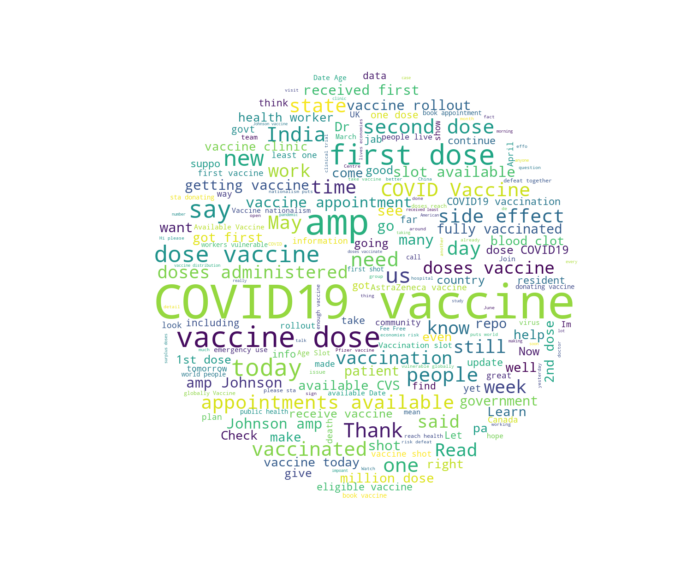
\includegraphics[width=0.65\linewidth]{resource/xinran/Word_Cloud.png}
  \caption{Word Cloud}
  \label{fig:wordcloud}
\end{figure}

\subsubsection{Topic Model Analysis}
~\\
Topic Modeling (TM) is an unsupervised technique for classifying documents in multiple themes. It consists of finding the information contained in textual documents and presenting it in the form of themes {\cite{topicmodeling}}. From the point of view of the representation space, the Topic Modeling is a reduction of dimensions in the vector representation of a document. Each value of this vector corresponding to the relative importance of the theme in this document. One example of topic modeling is Latent Dirichlet Allocation (LDA), which is used to extract themes from a document. In LDA models, each document is composed of multiple topics {\cite{LDA}}. We only consider tweets under the dominant topics obtained from the LDA model and then calculate the frequency of words based on tweets under each topic. There is some visualization work about the topic modeling (Figure~\ref{fig:2} \& Figure~\ref{fig:3}).
\begin{figure}[h]
  \centering
  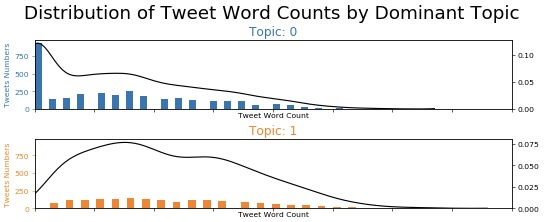
\includegraphics[width=0.65\linewidth]{resource/xinran/Word_Count_By_Topics.jpeg}
  \caption{Distribution of Tweet Word Counts by Dominant Topic}
  \label{fig:2}
\end{figure}

\begin{figure}[h]
  \centering
  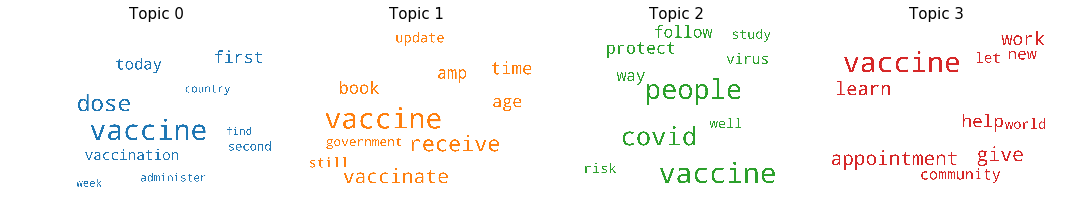
\includegraphics[width=\linewidth]{resource/xinran/TopKeywords_Topic.png}
  \caption{Word Clouds of Top N Keywords in Each Topic}
  \label{fig:3}
\end{figure}

\subsubsection{Sentiment Analysis Using VADER}
~\\
% Creating our own sentiment analysis model from scratch can be very difficult and tedious for a few reason. We need to find relevant data to your problem, create a lot of labeled data for training, and we must perform data clean up and NLP pre-processing. VADER is a readily available pre-trained sentiment analysis that thrives on social media data. So we use VADER to do the sentiment analysis.
Besides the above analysis, we also performed sentiment analysis for the dataset using the VADER. VADER (Valence Aware Dictionary and sentiment Reasoner) is a pre-trained lexicon and rule-based sentiment analysis tool that thrives on social media data. VADER utilizes a sentiment lexicon that is categorized as positive or negative based on its semantic orientation{\cite{vader}}. 

% The first analysis we are going to do is to plot a histogram of all of the sentiment scores we collected on our tweets as figure~\ref{fig:4}.
Figure~\ref{fig:4} is the histogram that represents the sentiment scores of each tweet in the dataset. Based on Figure~\ref{fig:4}, we can observe that the majority of tweets have a sentiment score of 0. In addition to neutral tweets, the proportion of positive tweets is larger than that of negative tweets.
\begin{figure}[h]
  \centering
  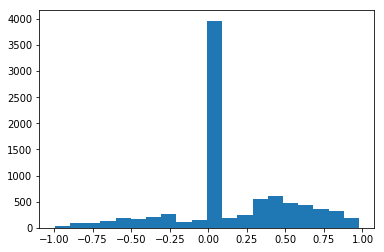
\includegraphics[width=0.65\linewidth]{resource/xinran/Sentiment_Analysis.png}
  \caption{Sentiment Analysis}
  \label{fig:4}
\end{figure}

% And we also plot a quick chart of our tweets and their sentiment over time as figure~\ref{fig:5}.
Figure ~\ref{fig:5} is a graph showing the change of sentiment of tweets over time.As seen in the Figure~\ref{fig:5}, the sentence score of tweets is continuously fluctuating based on time.
\begin{figure}[h]
  \centering
  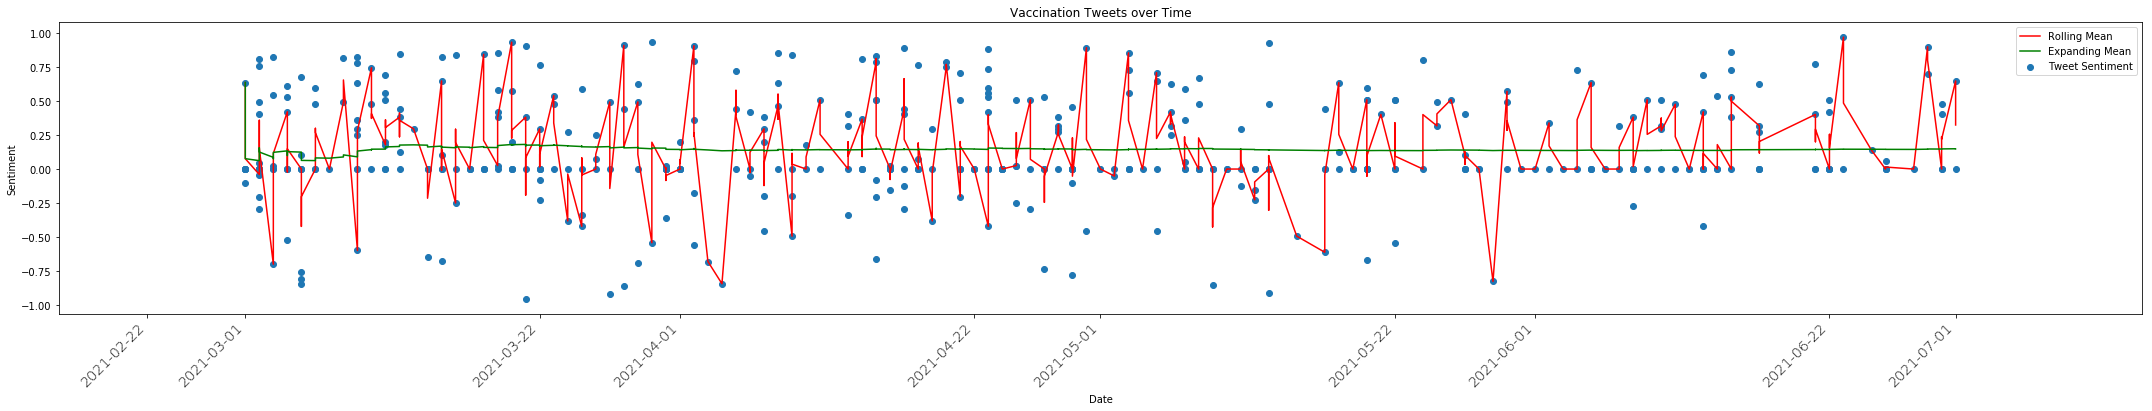
\includegraphics[width=1.0\linewidth]{resource/xinran/Vaccination_Tweets_over_Time.png}
  \caption{Vaccination Tweets over Time}
  \label{fig:5}
\end{figure}


\section{Methods}\label{methods}
In this section we will mainly describe the methods we used to build and partition the graph, then systematically considering
a variety of measures of homophily and controversy of the polarised communities within those networks.
\subsection{Graph Building}
In order to do analysis between communities we have to first build a tweet interaction graph and then partition it. The way we define a directed graph $G_d = (V,E)$, is that we treat each tweet as a node $V$, and the edge $E$ between each node is the relationships between the tweets. In this work, we choose retweets and mentions as the relationship between nodes to build our graph.

In addition to the unweighted graph $G_u$, We also uses dictionary-based sentiment analysis to do sentiment analysis of the texts of the tweets to generate a weighted graph $G_w$, and give the edge weights by the differences of sentiment between nodes. For each node, the sentiment of each node could be in the range of $[-1,1]$. The corresponding weight on the edge between nodes will be measured by the similarity of two sentiment scores.

In addition to the mentioned directed graph, we also generate a corresponding undirected graph for graph partitioning, which is because the algorithm we use does not work on directed graph.
\begin{figure}[h]
  \centering
  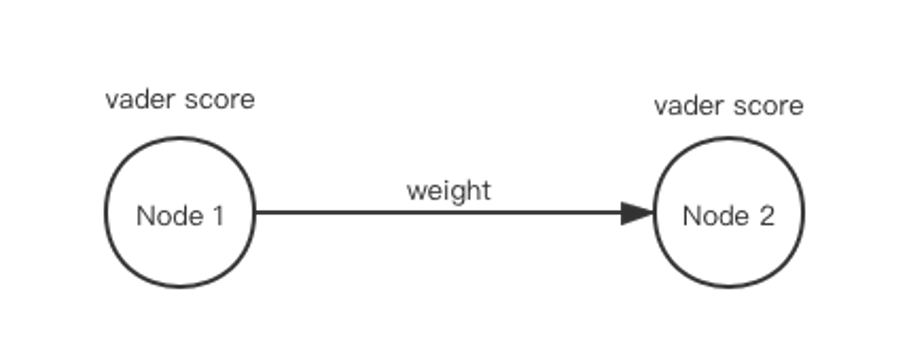
\includegraphics[width=0.85\linewidth]{resource/jiayi/nodes.png}
  \caption{Overall workflow of the METIS algorithm. }
\end{figure}

\subsection{Graph Partition}
To get the partitioned graph we used the METIS algorithm. In short it coarsens the graph to fewer nodes but still maintains the large structure, and keep this process until the graph is small enough. Then in the small graph we do a graph cut to split it into two communities. then with the partitioned small graph we map the value back to the refined larger maps.

However this method only works on undirected graph, so we transformed our directed graphs to undirected graph first, and then map it back to the directed graph for further analysis.
\begin{figure}[h]
  \centering
  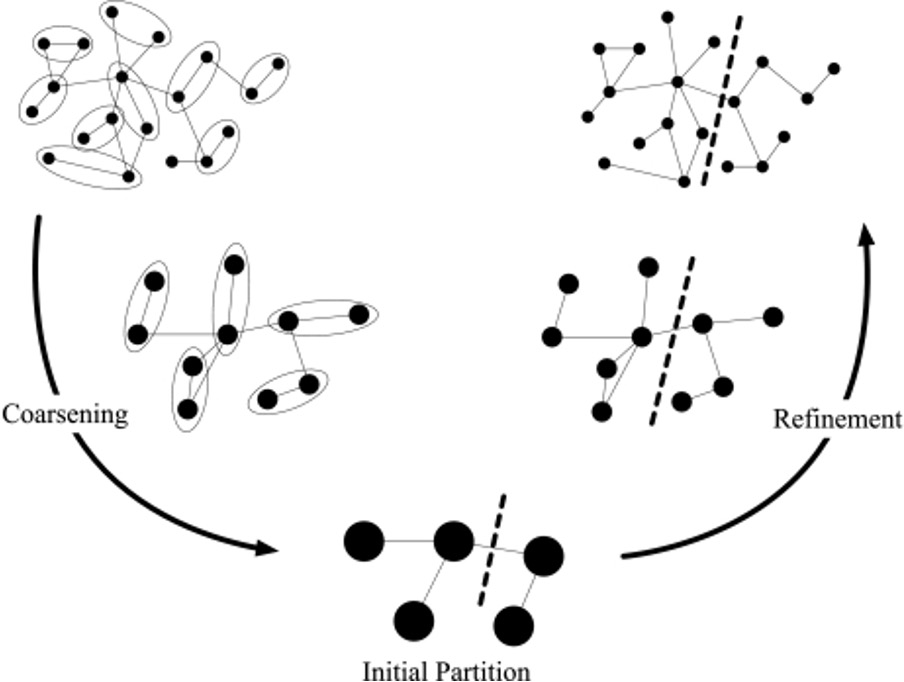
\includegraphics[width=0.85\linewidth]{resource/jiayi/metis.jpeg}
  \caption{Overall workflow of the METIS algorithm. }
\end{figure}

\subsection{Quantifying Polarization}
The last echo chamber detection phase consists in quantifying the polarization of the identified partitions, by assessing the goodness of community partition, controversy and homogeneity within them.

\subsubsection{Modularity and Coverage}
~\\
Modularity and coverage  {\cite{2004Finding}} {\cite{2009Community}} are the popular metrics to evaluate the goodness of community partition. They reflect the difference of a random network under a certain community partition. Specifically, the more edges inside the community and the fewer edges outside the community, the higher their value and the larger the corresponding difference, which means the better the community partition. However, these measures are used in most cases to quantify the results of community detection scenario. 

\subsubsection{Random Walk Controversy (RWC)}
~\\
For a comprehensive assessment of the echo chamber identification, we also apply Random Walk Controversy (RWC) {\cite{2015Quantifying}} to quantify the controversy in the networks. RWC is a measure of how controversial a topic discussed on social media is, i.e., how polarized a discussion it creates among the users, and it is usually considered in the identification of the echo chamber phenomenon. The formula is $$RWC = P_{XX}P_{YY} - P_{XY}P_{YX}$$ where X and Y are the two sides, and $P_{AB}$ is the probability of a random walker starting from $A$ to reach $B$.
It is a number in [0, 1] which represents the difference in probability for an average user in the network to be exposed to information from their own side versus from the opposing side. As such, RWC close to 1 represents a controversial topic with two communities that do not endorse each other’s opinion, while RWC close to 0 represents a non-controversial topic where both opinions are equally likely to be received.


\section{Results}
In this section we quantify the presence of echo chambers in each network, discuss their topological features, and show striking difference and interesting insights between two communities.

\subsection{Covid-19 Vaccine}
First, we focus on the big topic, this is, Covid-19 Vaccine, to explore the echo chamber effects. We analyze the distribution of attitudes and whether there was an echo chamber effect in the attitude choice of individuals when mentioning and replying on others’ tweets. 

\subsubsection{Community Structure}
~\\
Figure~\ref{fig:v} shows the mention and reply networks under the key word \textit{Covid-19 Vaccine}, constructed as explained in the \ref{methods} Method Section. (Each node’s size is proportional to its weighted in-degree, each line’s thickness was proportional to the edge’s weight, and each line’s color was consistent with the target node.)

Visually, we can observe that the networks are generally split into two communities of different color, which shows highly modular structures.

\begin{figure}[h]
  \centering
  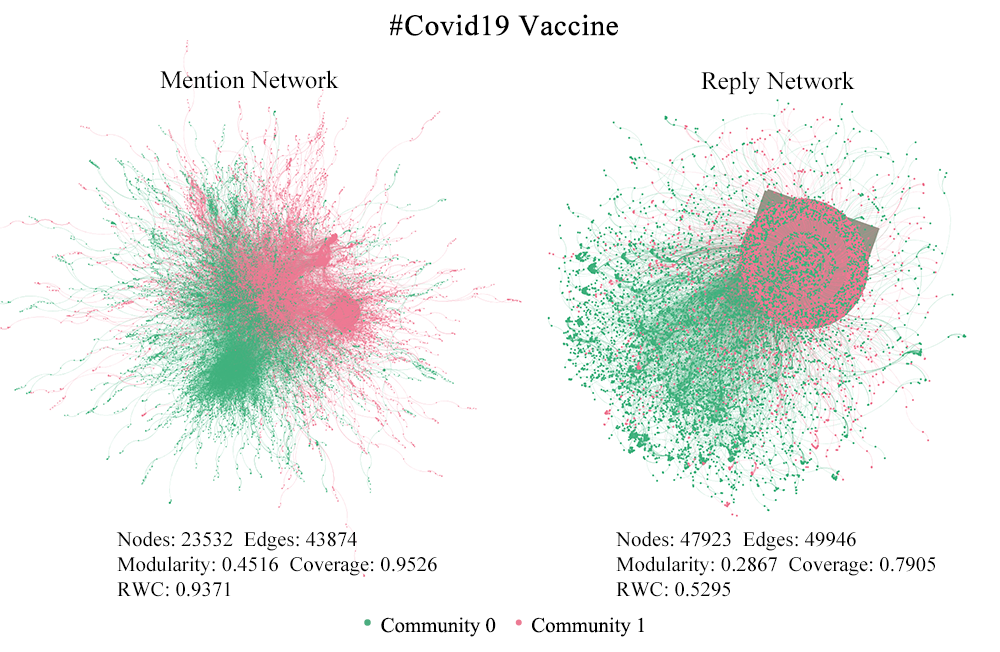
\includegraphics[width=0.9\linewidth]{resource/xiaoliang/v_m_r.png}
  \caption{The mention and reply networks of Covid-19 Vaccine.}
  \label{fig:v}
\end{figure}

From the results of evaluation metrics below each graph, we can see that the modularity and coverage values of mention network are all higher than reply network. Consequently, compared to reply, mention users created a more cohesive community and the relationship between users is closer and relatively more stable.

More specific, however, the large clusters in mention network showed high homophily, while the large clusters in reply network have some mixed attitudes. In the reply network, the structure of the two communities differs substantially. The community 0 (green part) is loose, whereas community 1 is dense showing a very tight relationship among it. But there are also some intermingled parts between the two communities. The fractured nature of the way users replying each other shows the lack of a coordinated effort and users in different communities are likely to reply each other to have a debate.

\subsubsection{Quantify Controversy}
~\\
The statistics of the mention and reply networks and RWC scores are shown in Table~\ref{tab: v_rwc}. The mention network shows a highly controversial topic, as indicated by the values of the RWC score, while the reply network shows a lower score, as it presents more connections across the two sides. 


\begin{table}
  \caption{Statistics of the mention and reply networks under topic \#Covid19 Vaccine: number of users $N$, number of edges $E$, number of users in two communities $N_0$ and $N_1$, Random Walk Controversy score $RWC$}
  \label{tab: v_rwc}
  \begin{tabular}{cccccl}
    \toprule
    Network & $N$ & $E$ & $N_0$ & $N_1$ & $RWC$\\
    \midrule
    Mention & 23532 & 43874 & 11451 & 12081 & 0.9371\\
    Reply & 47923 & 49946 & 23242 & 24618 & 0.5295\\
  \bottomrule
\end{tabular}
\end{table}


\subsection{Sinovac and Pfizer Vaccine}
To take a more nuanced look at people's attitudes toward vaccines, we also explored echo chambers based on the discussions of \textit{Pfizer} and \textit{Sinovac vaccines} separately. We examined the content of user interaction from the dimension of sentiment expression, and civility to test the impact of the echo chamber effect. Based on the results at user and community levels, we made a comprehensive judgment.

\subsubsection{Community Structure}
~\\
Figure~\ref{fig:s} and Figure~\ref{fig:p} show the mention and reply networks under the key word $Sinovac$ and $Pfizer$. To some extent, the basic community structures of networks are consistent with the networks under the topic of \textit{Covid-19 Vaccine} generally, this is, the reply network have one loose cluster and one dense cluster, while the structure of two sides in mention network are more similar. The difference is that the mention interactions between users are more frequent and tighter under specific vaccine topic. That means a more detailed topic tend to trigger more discussions and debates.

\begin{figure}[h]
  \centering
  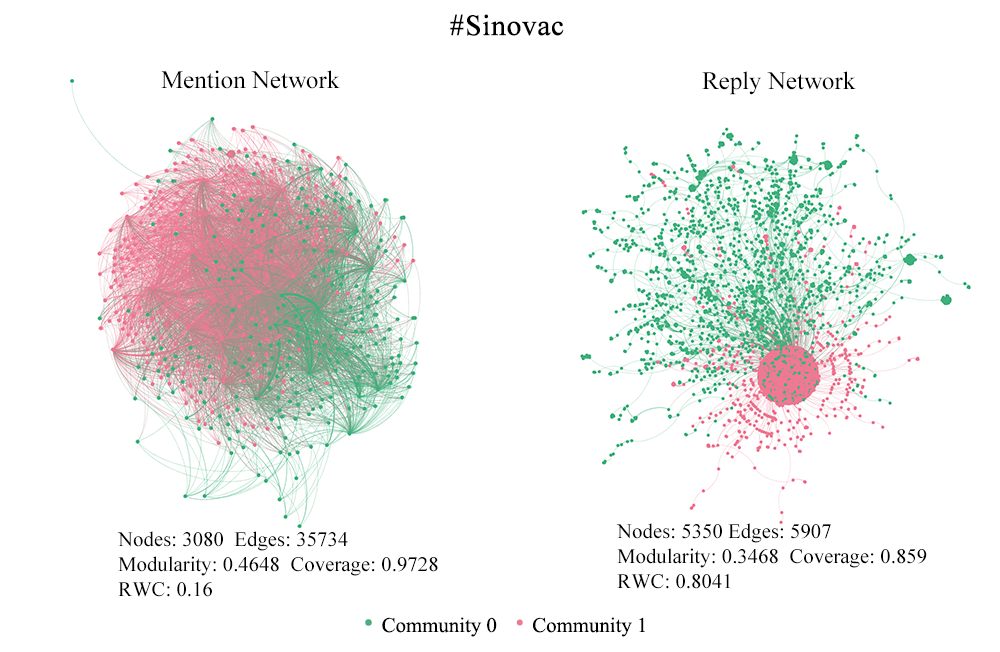
\includegraphics[width=0.9\linewidth]{resource/xiaoliang/s_m_r.png}
  \caption{The mention and reply networks of Sinovac Vaccine.}
  \label{fig:s}
\end{figure}

\begin{figure}[h]
  \centering
  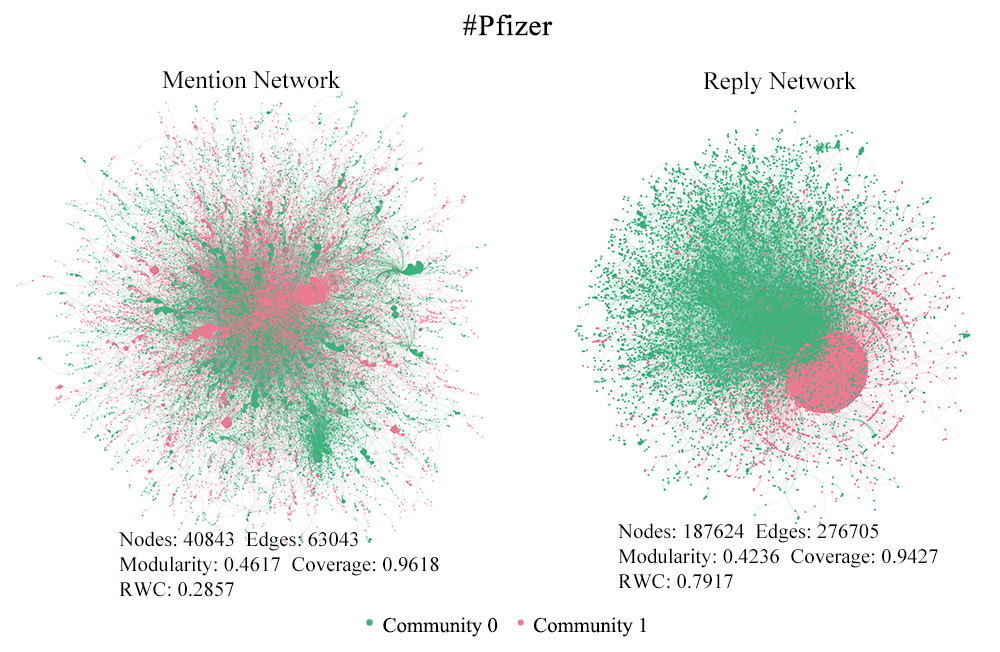
\includegraphics[width=0.9\linewidth]{resource/xiaoliang/p_m_r.png}
  \caption{The mention and reply networks of Pfizer Vaccine.}
  \label{fig:p}
\end{figure}


\subsubsection{Quantify Controversy}
~\\
On the other hand, the RWC results in Table~\ref{tab: s_rwc} and Table~\ref{tab: p_rwc} also show some different insights. Since reply is often used to speak to (and attack) the opposing side. The reply networks show a highly controversial topic. 

\begin{table}
  \caption{Statistics of the mention and reply networks under topic \#Sinovac: number of users $N$, number of edges $E$, number of users in two communities $N_0$ and $N_1$, Random Walk Controversy score $RWC$}
  \label{tab: s_rwc}
  \begin{tabular}{cccccl}
    \toprule
    Network & $N$ & $E$ & $N_0$ & $N_1$ & $RWC$\\
    \midrule
    Mention & 3080 & 35734 & 1496 & 1584 & 0.16\\
    Reply & 5350 & 5907 & 2755 & 2595 & 0.8041\\
  \bottomrule
\end{tabular}
\end{table}

\begin{table}
  \caption{Statistics of the mention and reply networks under topic \#Pfizer: number of users $N$, number of edges $E$, number of users in two communities $N_0$ and $N_1$, Random Walk Controversy score $RWC$}
  \label{tab: p_rwc}
  \begin{tabular}{cccccl}
    \toprule
    Network & $N$ & $E$ & $N_0$ & $N_1$ & $RWC$\\
    \midrule
    Mention & 40843 & 63043 & 20595 & 20248 & 0.2857\\
    Reply & 187624 & 276705 & 95321 & 92303 & 0.7917\\
  \bottomrule
\end{tabular}
\end{table}

\subsubsection{Sentiment Analysis}
~\\
On the basis of the analysis above, we continue to dig deeper into the sentiment analysis of echo chambers in communities based on reply networks. Sentiment analysis for communities includes two aspects, the percentage of tweets with different polarities, and word cloud diagrams for positive and negative tweets.

Under \textit{Sinovac topic}, there are two important findings for two communities in Figure \ref{fig:pola_sinovac}. The proportion of neutral and positive tweets exceeds 85\% and more than 45\% of tweets are in the neutral category which has the largest percentage. Therefore the majority of people are not vaccination skeptics and are neutral about the Sinovac vaccine. The polarity proportions of two echo chambers built on reply networks are generally similar except that community 1 has a larger proportion of vaccine skeptics. 

\begin{figure}[h]
  \centering
  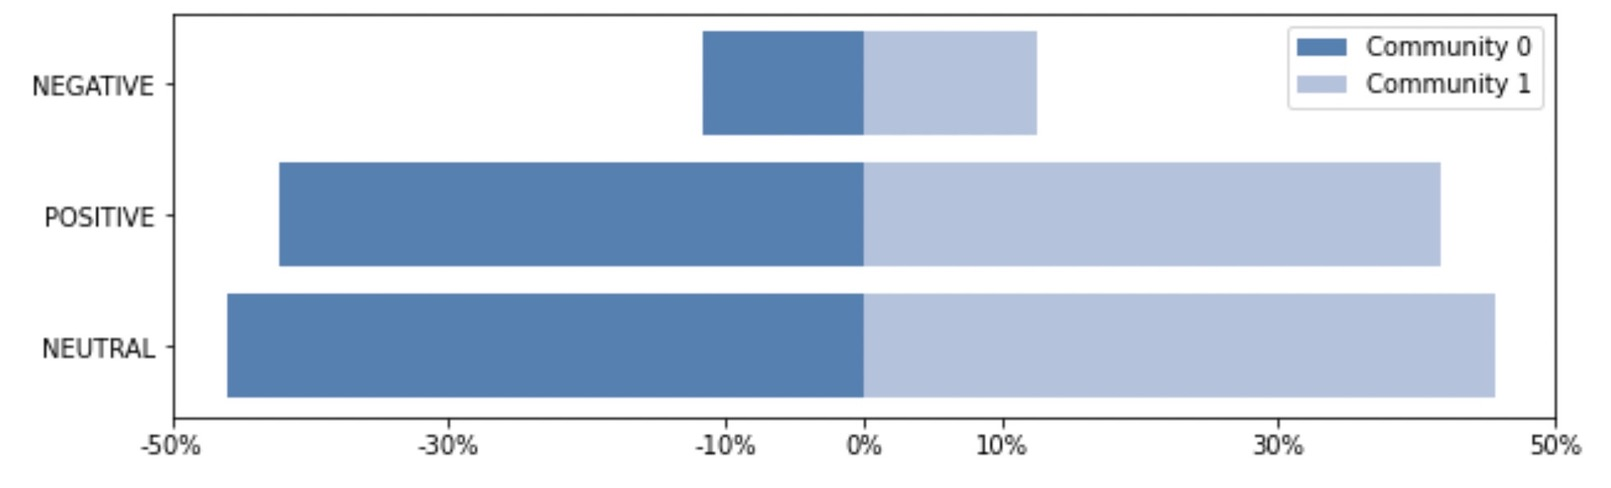
\includegraphics[width=0.8\linewidth]{resource/yidan/sinovac_sentiment2.jpeg}
  \caption{The percentage of tweets with different polarity in Sinovac vaccine.}
  \label{fig:pola_sinovac}
\end{figure}

\begin{figure}[h]
  \centering
  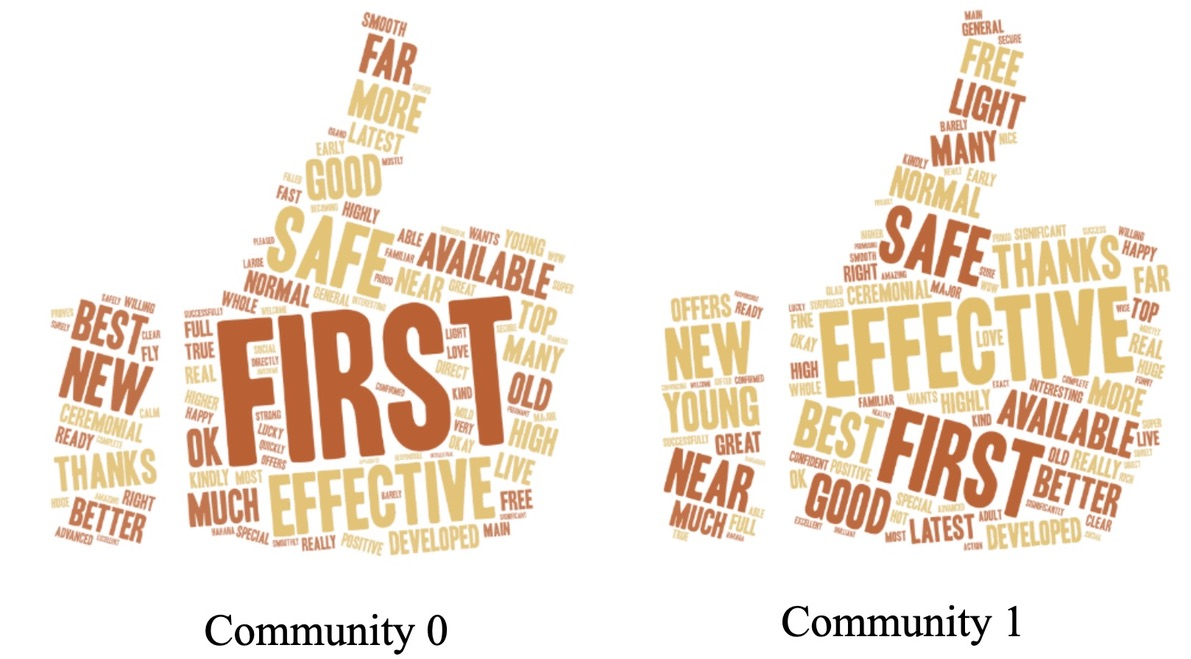
\includegraphics[width=0.6\linewidth]{resource/yidan/Sinovac_wc_pos.jpeg}
  \caption{Word cloud diagram of positive tweets for Sinovac vaccine.}
  \label{fig:wc_pos_Sinovac}
\end{figure}

After analysis of polarity proportions, the word cloud diagrams are constructed using TF-IDF {\cite{tfidf}} and TextBlob{\cite{textblob}} techniques. For both communities, the keywords that people valued in the positive tweets are overall similar (Figure \ref{fig:wc_pos_Sinovac}). “First”, ”Effective” and “Safe” are words with large percentages. However, there are some differences. The most significant word in Community 0 is "First." In comparison, "Effective" has the largest proportion in Community 1. Because the data ranges from 1 March 2021 to 1 July 2021. At that time, the vaccine had been available to people and the majority of people had received their first dose. Hence the high frequency of "First" and "Effective" is reasonable.

\begin{figure}[h]
  \centering
  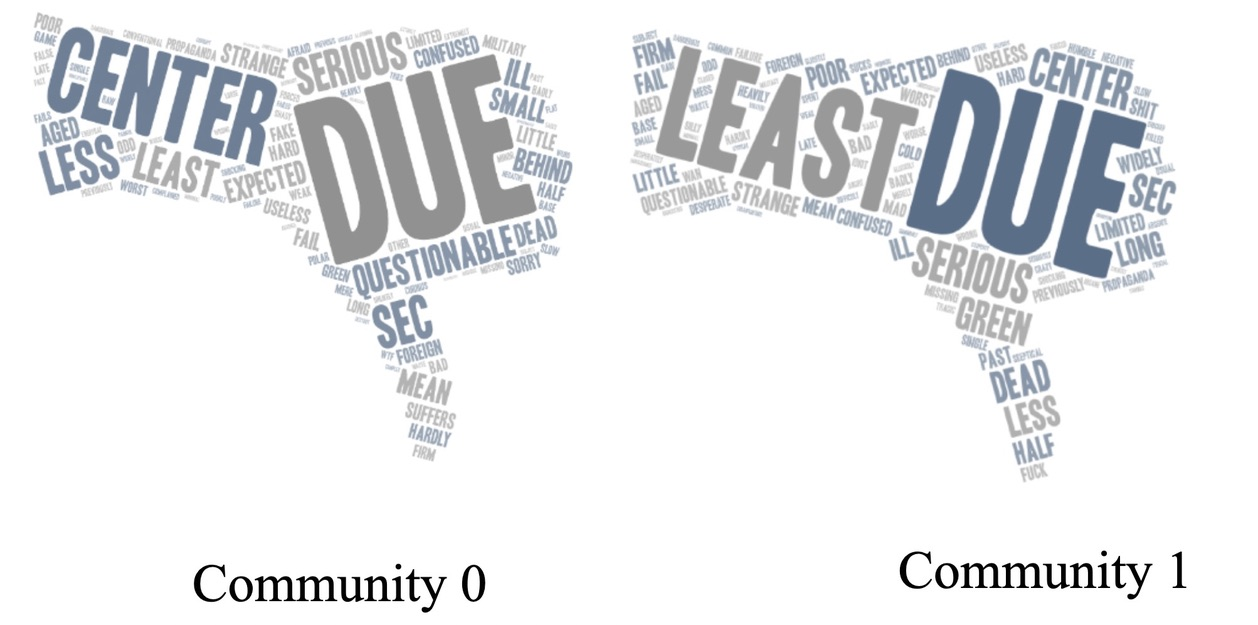
\includegraphics[width=0.6\linewidth]{resource/yidan/Sinovac_wc_neg.jpeg}
  \caption{Word cloud diagram of negative tweets for Sinovac vaccine.}
  \label{fig:wc_neg_Sinovac}
\end{figure}

Figure \ref{fig:wc_neg_Sinovac} shows the word cloud diagram in negative tweets. Three most essential words in two communities are “Least”, “Due” and “Center”. However, there are some distinctions between two communities with people in Community 0 valuing “Due” and “Center”. Nevertheless, “Due” and “Least” are more important in Community 1. In most of the negative tweets, “Due” is used in “Due to Sinovac vaccines” to refer to the source of the side effects,  “Least” is used in “At least some people” to describe the number of people involved in the side effects and “Center” is mainly used to specify the center where the Sinovac vaccine was administered.

Besides Sinovac topics, \textit{Pfizer topics} are also analyzed. Two essential findings of the two communities can be obtained in Figure \ref{fig:pola_pfizer}. More than 84\% of tweets belong to positive and neutral and more than 50\% of people have a positive attitude. Therefore, we can conclude that these findings are similar to that of the Sinovac topic, only a small percentage of people are vaccination skeptics. But compared to a neutral attitude towards Sinovac vaccines, most people have a positive attitude to the Pfizer vaccines.

\begin{figure}[h]
  \centering
  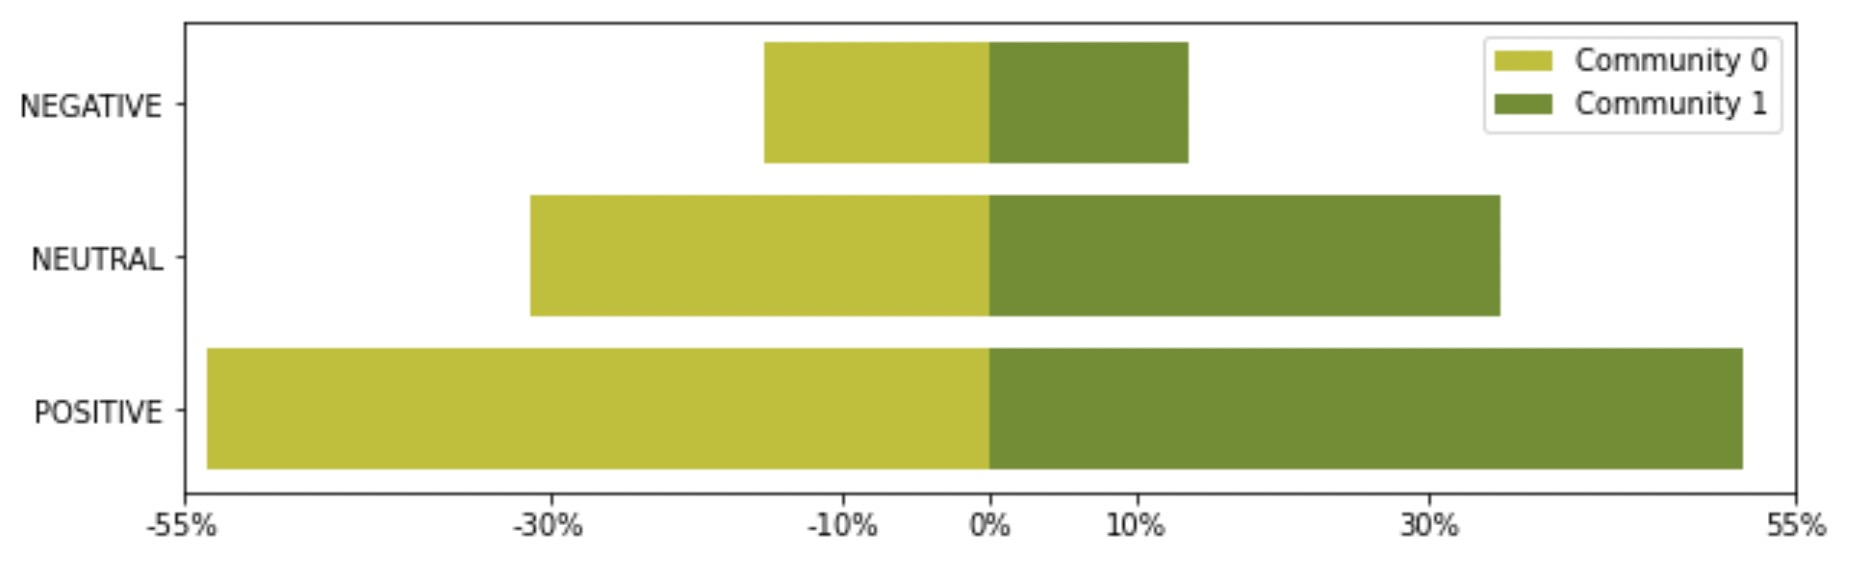
\includegraphics[width=0.8\linewidth]{resource/yidan/Pfizer_sentiment2.jpeg}
  \caption{The percentage of tweets with different polarity in Pfizer vaccine.}
  \label{fig:pola_pfizer}
\end{figure}

\begin{figure}[h]
  \centering
  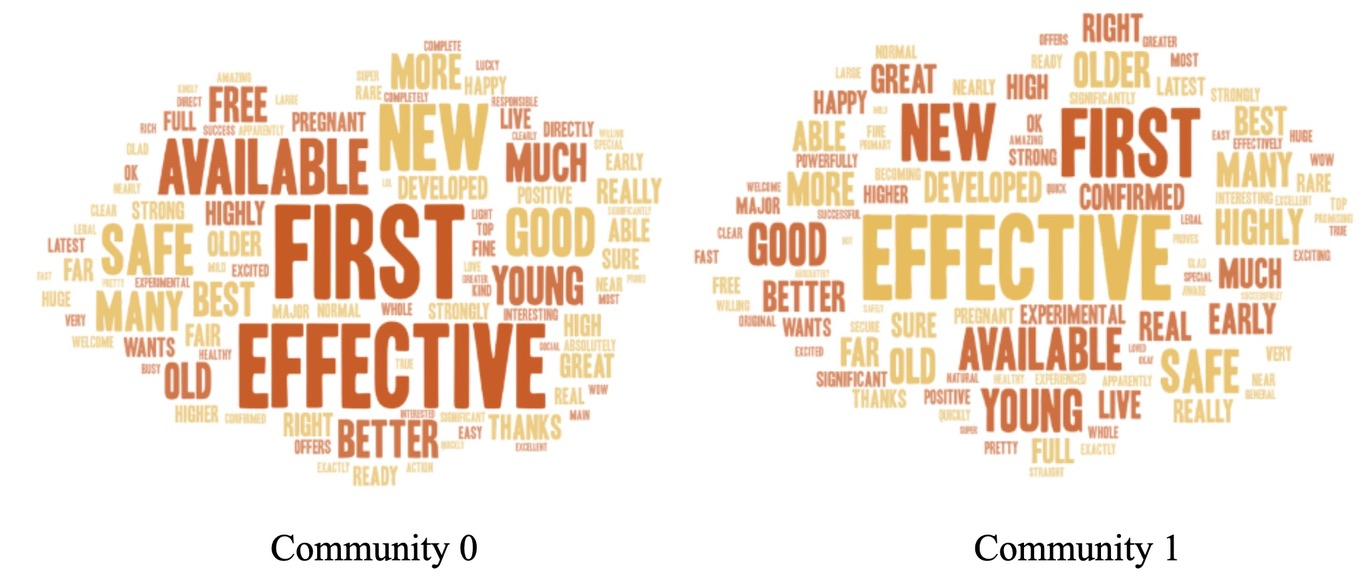
\includegraphics[width=0.6\linewidth]{resource/yidan/Pfizer_wc_pos.jpeg}
  \caption{Word cloud diagram of positive tweets for Pfizer vaccine.}
  \label{fig:wc_pos_Pfizer}
\end{figure}

\begin{figure}[h]
  \centering
  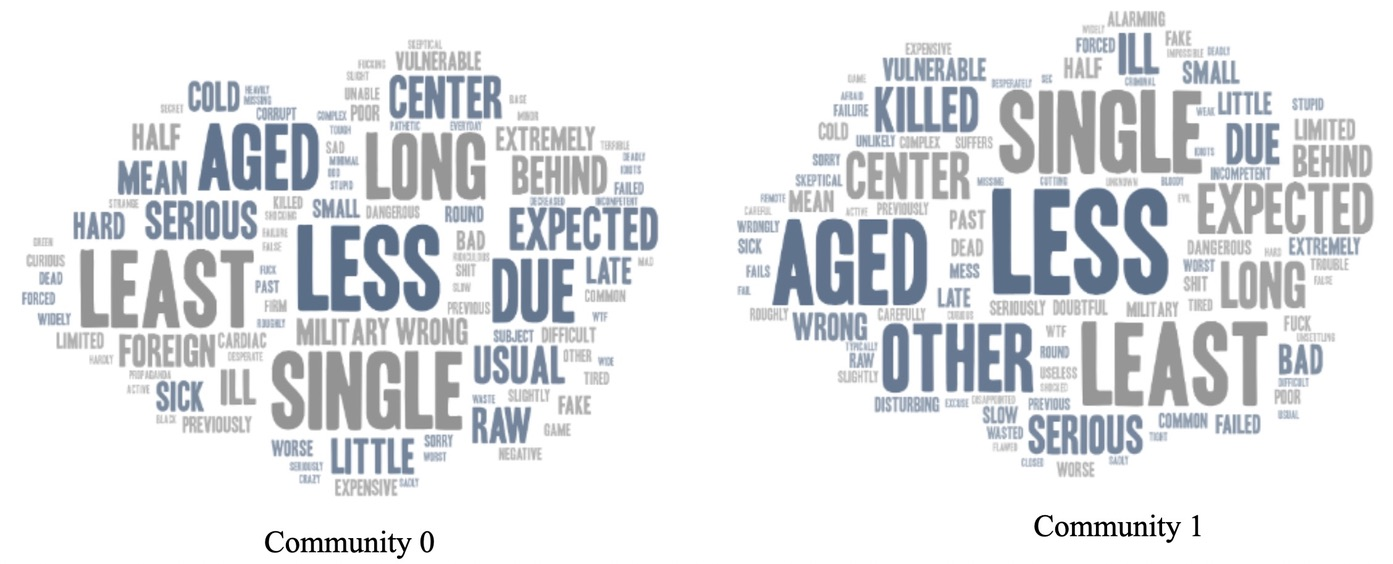
\includegraphics[width=0.6\linewidth]{resource/yidan/Pfizer_wc_neg.jpeg}
  \caption{Word cloud diagram of negative tweets for Pfizer vaccine.}
  \label{fig:wc_neg_Pfizer}
\end{figure}

For the Pfizer topic, two most important words for the Pfizer vaccine are “First” and “Effective” (Figure \ref{fig:wc_pos_Pfizer}), which is similar to the Sinovac topic. After exploration of relevant tweets, “First” is frequently referred to as “First vaccine” since most people get their first dose of the vaccine around that time. “Effective” mainly indicates the concerns of people about the effectiveness of vaccinations. There are some distinctions between the two communities. “First” is the most crucial word in Community 0. Whereas, “Effective” has the largest proportion in Community 1. 

Figure \ref{fig:wc_neg_Pfizer} shows the word cloud diagrams of negative tweets. It is different from the figure on the Sinovac topic (Figure \ref{fig:wc_neg_Sinovac}). “Single” and “Less” are the two most essential words in the two communities. “Single” is mentioned more frequently in Community 0. “Less” has the largest proportion in Community 1. “Single” is often used for “Single vaccination” to describe the side effects of a single vaccine. “Less” is usually referred to indicate that a single vaccine can only provide limited protection against the virus.

\subsubsection{Centers of Communities}
~\\
After the sentiment analysis of echo chambers in communities, we continue to explore the centers of the communities in the reply network, this is, the nodes with higher degree, to further explore the echo chamber effect.
% On the basis of sentiment analysis above, we continue to dig deeper on the topology of echo chambers in communities. Hence, we find the centers of the communities in the reply network, this is, the nodes with higher degree, to further explore the echo chamber effect.

Under the \textit{Sinovac topic}, the centers of community 1 are some news media accounts related to China, like @cnnphilippines, @sinovac, @BridgeBeijing. In community 0, we find some news and journalists accounts most from all over the world, like @VOAStevenson, @Reuters, @inquieredotnet @ABSCBNNews, @Nepal\_News\_En. This may indicate that users of community 0 are more likely to be distributed all around the world, which contain various attitudes and opinions, while users of community 1 are more concentrated in or related to China, and their attitudes towards Sinovac will be relatively positive, hence, leading to a tighter relationship in the community. The results match the topological features of network graph in Figure~\ref{fig:s}.

Under the \textit{Pfizer topic}, from the centers of community 1, we find @EricTopol (a physician scientist, author, editor with 600 thousands followers) and @PLHartungRN (Retired VP of Pfizer vaccines). Both of them are supportive or neutral of the Pfizer vaccine. While in community 0, we find @ExmoorOn (Retired immunologist, focus on biotechnology mRNA) and @KathMLee1 (PhD research on chemistry and biology). They are quite critical about Pfizer vaccine since both of them posted some articles and tweets on Pfizer’s side effect. The results also match the reply network graph in Figure~\ref{fig:p}. The distribution of users in community 1 is concentrated, in contrast, community 0 is divergent.



\section{Conclusion}
~\\
In this project, we achieved two goals by constructing and analyzing the echo chambers in the context of covid-19 vaccinations. 
The first goal is to analyze the attitudes in the echo chambers towards vaccines. We found that more than 80\% of people have a positive or neutral attitude towards the covid-19 vaccine, and only a small proportion of people are vaccine skeptics. The second goal is to identify potential rumor spreaders, that is centers of rumor echo chambers. There are some rumor spreaders detected. @3\textasciitilde VaccineInjuries.ca send many tweets to spread vaccine side effects. @Toby Young and @Kyle Becker spread some rumors related to vaccine efficacy. Their tweets were widely disseminated and even mentions and replies of tweets include many vaccine rumors. Additionally, certain methods are investigated to intervene in the propagation of rumors. Firstly, the most straightforward way is to detect the centers of rumor echo chambers and interfere with them to halt the rumor spread. Secondly, some tools (like a Gamified Inoculation System {\cite{chamberbreaker}} ) have been proven to be effective in interfering with echo chamber propagation. In addition to the measures for rumor spreaders, message recipients (all of us) should learn to identify and get out of an echo chamber. There are three practical suggestions. Firstly, it is essential to check multiple news sources, especially authoritative media. The second way is to turn off personalized recommendations in social media applications to obtain a variety of information. Thirdly, it is vital to converse with people who have opposing views, which can help you to receive more diverse and extensive information {\cite{getoutofec}}.
~\\
This project has three contributions. Firstly, we crawled the data to construct our own dataset through keywords \#Covid19\_vaccine, \#Pfizer, \#Sinovac, and two time periods Mar 01, 2021 - Jul 01, 2021 and Dec 01, 2021 - Mar 01, 2022. The second aspect is to construct 12 echo chambers based on explicit relationships including mention and reply. The third aspect is to analyze echo chambers and explore some meaningful findings. 



% Therefore, we want to discuss why the echo chamber occurs. We think there are three reasons.The first is that the individual belief system tends to gather information that support their existing beliefs. The second is that personalized algorithms will recommend the specific information. Thirdly, the characteristic of echo chamber means that people are not fully responsible for their convictions.
% Then I want to talk about how to get out of an echo chamber. There are three suggestions. When we obtain information, we should check multiple news sources especially authoritative media. The second is to turn off personalized recommendation to obtain a variety of different information. The third one is to discuss with people who have different view from you.


% --------------------------------------------------------------




% \section{Math Equations}
% You may want to display math equations in three distinct styles:
% inline, numbered or non-numbered display.  Each of the three are
% discussed in the next sections.

% \subsection{Inline (In-text) Equations}
% A formula that appears in the running text is called an inline or
% in-text formula.  It is produced by the \textbf{math} environment,
% which can be invoked with the usual
% \texttt{{\char'134}begin\,\ldots{\char'134}end} construction or with
% the short form \texttt{\$\,\ldots\$}. You can use any of the symbols
% and structures, from $\alpha$ to $\omega$, available in
% \LaTeX~\cite{Lamport:LaTeX}; this section will simply show a few
% examples of in-text equations in context. Notice how this equation:
% \begin{math}
%   \lim_{n\rightarrow \infty}x=0
% \end{math},
% set here in in-line math style, looks slightly different when
% set in display style.  (See next section).

% \subsection{Display Equations}
% A numbered display equation---one set off by vertical space from the
% text and centered horizontally---is produced by the \textbf{equation}
% environment. An unnumbered display equation is produced by the
% \textbf{displaymath} environment.

% Again, in either environment, you can use any of the symbols and
% structures available in \LaTeX\@; this section will just give a couple
% of examples of display equations in context.  First, consider the
% equation, shown as an inline equation above:
% \begin{equation}
%   \lim_{n\rightarrow \infty}x=0
% \end{equation}
% Notice how it is formatted somewhat differently in
% the \textbf{displaymath}
% environment.  Now, we'll enter an unnumbered equation:
% \begin{displaymath}
%   \sum_{i=0}^{\infty} x + 1
% \end{displaymath}
% and follow it with another numbered equation:
% \begin{equation}
%   \sum_{i=0}^{\infty}x_i=\int_{0}^{\pi+2} f
% \end{equation}
% just to demonstrate \LaTeX's able handling of numbering.

%%
%% The next two lines define the bibliography style to be used, and
%% the bibliography file.
\bibliographystyle{ACM-Reference-Format}
\bibliography{ref}

\end{document}
\endinput
%%
%% End of file `sample-sigplan.tex'.
